\documentclass[colorBG,slideColor,9pt]{beamer}
\mode<presentation>
{
  % Use the IIS-theme
  \usetheme{FHL}
  % Der mathematische Schriftsatz ist mit Serifen
  \usefonttheme[onlymath]{serif}
  % Noch nicht aufgedeckte Punkte erscheinen ausgegraut
%  \setbeamercovered{transparent}
  % Bild-/Tabellen�berschriften sind sehr klein
  \setbeamerfont{caption}{size=\tiny}
}
%\usepackage[german]{babel}
\usepackage[utf8]{inputenc}
\usepackage{amsmath,bm}
\usepackage[]{easymovie}
\usepackage{helvet} 
\usepackage{setspace}
\renewcommand{\familydefault}{\sfdefault}
%
% Dick der Folientitel 1. Folie
%
\newcommand{\talktitle}{�ber den Unsinn der Steuergesetzgebung} 
%
% Some useful macros:
\newcommand{\MatDef}[2]{\left[ \hspace{-0.4em} \begin{array}{#1} #2 \end{array} \hspace{-0.4em} \right]}
\newcommand{\E}[1]{\ensuremath{\mathrm{E}\hspace{-0.12em}\left\{#1\right\}}}
\newcommand{\real}[1]{\ensuremath{\mathrm{Re}\hspace{-0.12em}\left\{#1\right\}}}
\newcommand{\imag}[1]{\ensuremath{\mathrm{Im}\hspace{-0.12em}\left\{#1\right\}}}
\newcommand{\ex}[1]{\ensuremath{e^{#1}}}
\newcommand{\si}[1]{\ensuremath{\mathrm{si}\left(#1\right)}}
\newcommand{\rect}[1]{\ensuremath{\mathrm{rect}\left(#1\right)}}
\newcommand{\tri}[1]{\ensuremath{\mathrm{tri}\left(#1\right)}}
\newcommand{\mycos}[1]{\ensuremath{\cos{\left(#1\right)}}}
\newcommand{\mysin}[1]{\ensuremath{\sin{\left(#1\right)}}}
\newcommand{\corrbone}{\quad  \mbox{$\circ$  \hspace{-0.65em} --- \hspace{-0.65em}  $\bullet$}  \quad}
\newcommand{\invcorrbone}{\quad  \mbox{$\bullet$  \hspace{-0.65em} --- \hspace{-0.65em}  $\circ$}  \quad}
\newcommand{\maker}[1]{\textcolor{red!80!black}{#1}}
\newcommand{\makeg}[1]{\textcolor{green!74!black}{#1}}
\newcommand{\makeb}[1]{\textcolor{blue!80!black}{#1}}
%
% -----------------------------------------------------------
% Begin
% -----------------------------------------------------------
\begin{document}
% -----------------------------------------------------------
% Title page
% -----------------------------------------------------------
\begin{frame}
    \vspace{-10ex}
    \textcolor{fhlred}{\HRuleFill[0.4ex]} \\ \vspace{1ex}
    {\linespread{1.5}\selectfont
    \MakeUppercase{\bf \huge \talktitle}\\[5.5ex]}
    \normalsize Eine frustrierte Erkenntnis\\
    \textcolor{fhlred}{\HRuleFill[0.1ex]} \\ \vspace{4ex}
    \small Max Meier\\
    \small Fachschule L�beck, demn�chst Technische Hochschule L�beck\\
    \vspace{2ex}
    \small Angefertigt bei\\
    \small Bedeutendes Unternehmen (nach eigener Aussage)
\end{frame}


% ----------------------------
%   Section Inhalts�bersicht
% ----------------------------

\section{Kapitel}
\begin{frame}[fragile]
\frametitle{Gliederung}
\vspace{4.0ex}
Eine Aufz�hlung:
\begin{enumerate}
\itemsep 2.0ex
\item  Erster Eintrag
\begin{itemize}
\item  Erster Untereintrag
\item  Zweiter Untereintrag
\end{itemize}
\item[]  $\Rightarrow$ Kann man machen.
%
\item Muss man aber nicht.
\end{enumerate}
\end{frame}

% ----

\begin{frame}
\frametitle{Einbindung einer Grafik}

\begin{center}
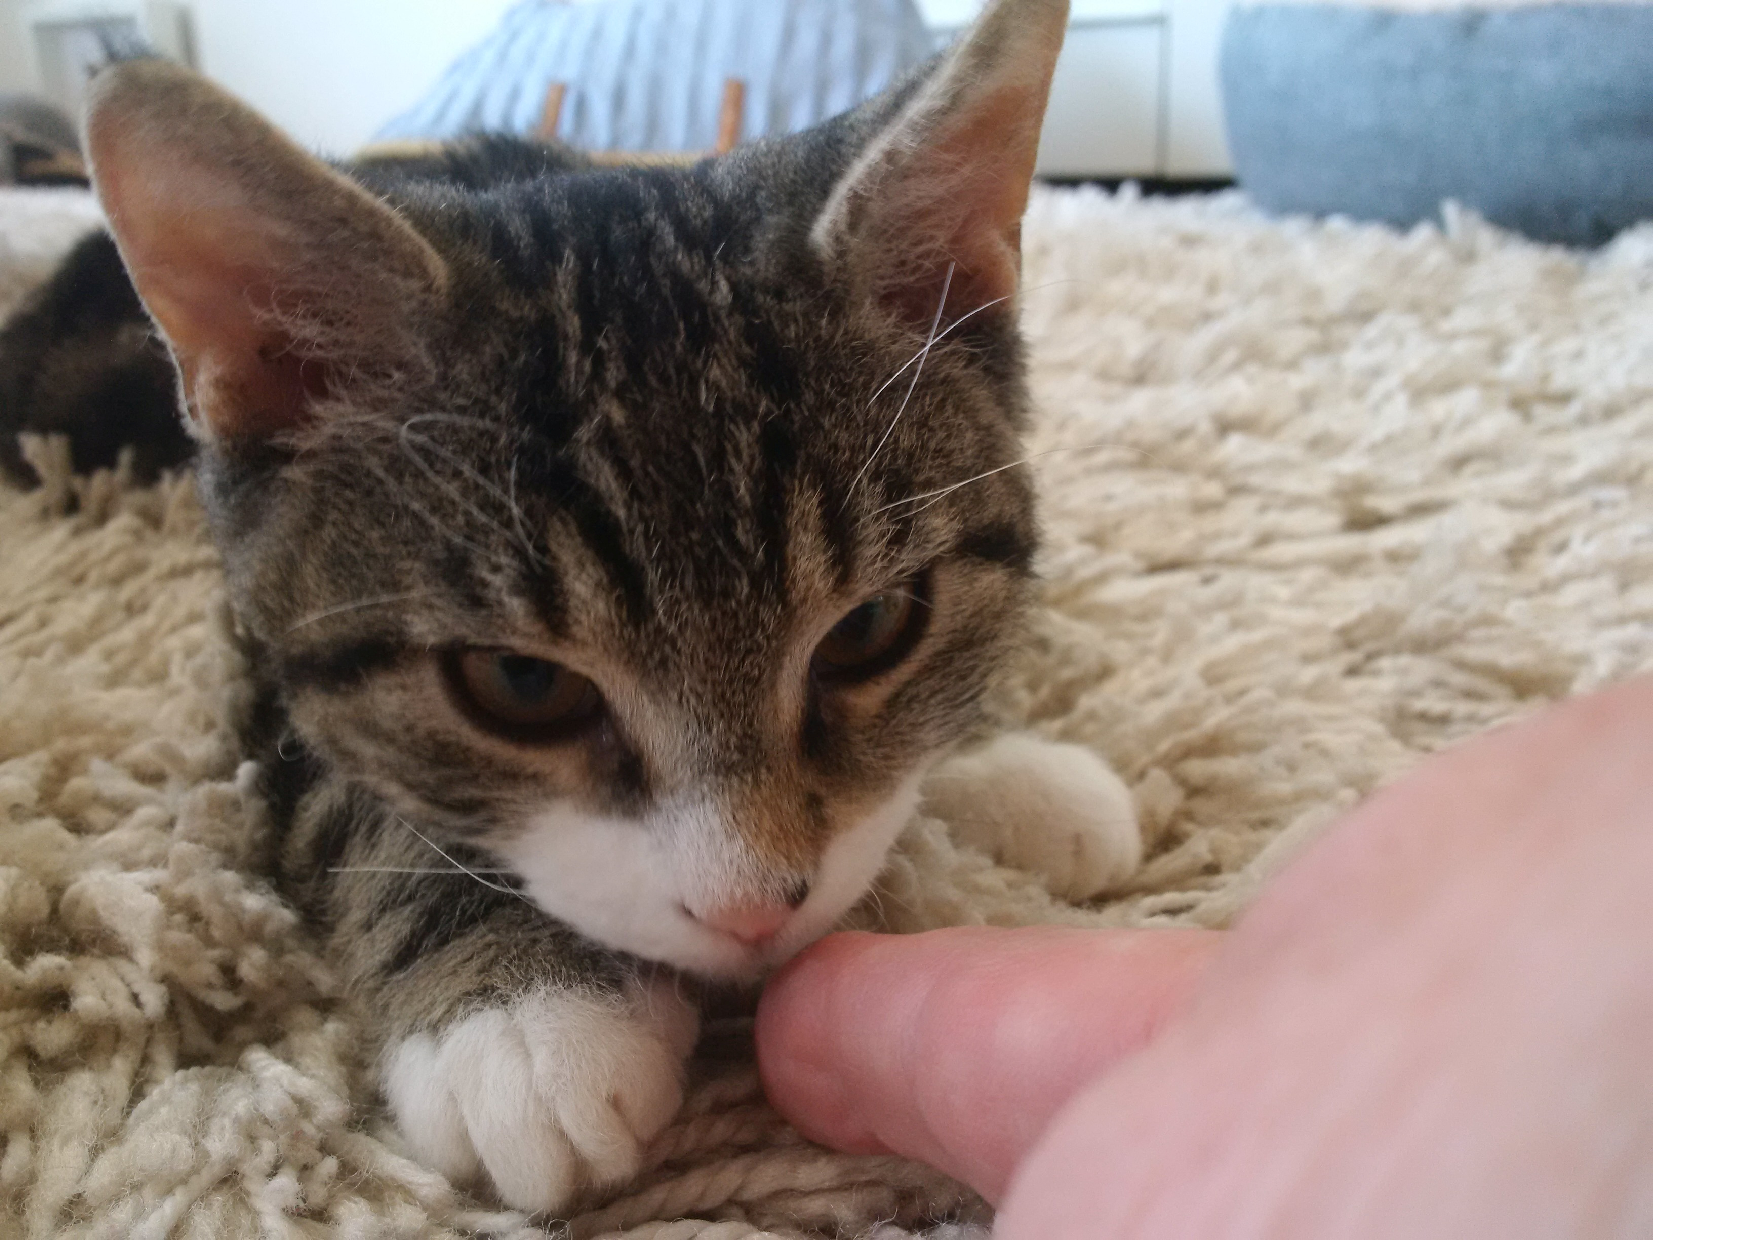
\includegraphics[width=9cm]{figs/UllisKater.pdf}
\end{center}

\end{frame}

% -----------------------------------------------------------
% End
% -----------------------------------------------------------

\end{document}
